\section{Theorie}
\label{sec:Theorie}

Der Photoeffekt ist ein Phänomen, das den Teilchencharakter von Lichtwellen aufzeigt.
Dieses Phänomen ist zu beobachten, wenn eine Metalloberfläche mit Licht bestrahlt wird.
Durch die Wechselwirkung mit den Elektronen auf der Metalloberfläche übertragen  Photonen --
quantitisierte Teilchen -- ihre Energie $E_{\mathrm{Photon}}$ an diese.
Dies führt zu einem Austritt der Elektronen, wenn die Elektronen eine genügend große Energie
besitzen, um die Austrittsarbeit $A_{\mathrm{k}}$ zu verrichten, die nötig ist, um die
Bindungskräfte zu überwinden.

Die experimentellen Beobachtungen des Photoeffekts liefern drei grundlegende Ergebnisse.
Zum Einen ist die Auslösefrequenz der Elektronen proportional zur Lichtintensität.
Des Weiteren ist die Energie der ausgelösten Elektronen proportional zur Frequenz des Lichtes
und nicht abhängig von der Lichtintensität.
Und außerdem gibt es eine Lichtfrequenz, ab der -- aufgrund der zu geringen Energie -- kein
Photoeffekt auftritt.

Diese Ergebnisse lassen sich nicht mit einem Wellenmodell erklären, bei dem die Elektronen
durch das elektrische Feld der elektromagnetischen Wellen zu Schwingungen  angeregt werden.
Dann müsste die Anzahl der ausgelösten Elektronen von der Intensität des Lichtes abhängen
und es müssten Resonanzeffekte auftreten.

Da dies nicht der Fall ist, lässt sich der Photoeffekt nur durch den Teilchencharakter des
Lichtes erklären, also durch die sogenannten Lichtquanten oder Photonen.
Die drei grundlegenden Ergebnisse haben drei experimentell belegte Gründe, die auf dem
Teilchencharakter des Lichtes basieren.

Zum Einen besitzen Photonen -- bei monochromatischem Licht -- die Energie
\begin{equation}
	E_{\mathrm{Photon}} = \symup{h} \nu \mathrm{,}
\end{equation}
wobei $\symup{h}$ dem Planck'schen Wirkungsquantum und $\nu$ der Frequenz des Lichtes
entspricht.
Des Weiteren ergibt sich die Energiebilanz zu
\begin{equation}
	\label{eqn:energybalance}
	\symup{h} \nu = E_{\mathrm{kin}} + A_{\mathrm{k}} \mathrm{,}
\end{equation}
mit der kinetischen Energie $E_{\mathrm{kin}}$ eines Elektrons nach dem Austritt aus der
Metalloberfläche.
Die Existenz einer Grenzfrequenz, ab der kein Photoeffekt mehr auftritt, folgt direkt aus
Formel \eqref{eqn:energybalance} mit
\begin{equation*}
	\symup{h} \nu < A_{\mathrm{k}} \mathrm{.}
\end{equation*}
Die Energie der ausgelösten Elektronen wird experimentell mit einer Gegenfeldmethode bestimmt.
Hierbei müssen die ausgelösten Elektronen auf dem Weg zur Anode, von wo aus sie zu einem
Strommessgerät gelangen, ein durch eine variable Spannung $U$ bedingtes Gegenfeld
durchqueren. Daraus folgt, dass kein Strom gemessen werden kann, wenn die kinetische Energie
der schnellsten Elektronen der Energie entspricht, die nötig ist, um das Gegenfeld zu
durchlaufen, wenn also
\begin{equation}
	\symup{e}_0 \, U_{\mathrm{g}} = \frac{1}{2} \symup{m}_0 \, v_{\mathrm{max}}^2
\end{equation}
gilt. Die Spannung $U_{\mathrm{g}}$, bei der dieser Zusammenhang gegeben ist, heißt
Gegenspannung. Des Weiteren entspricht das $\symup{e}_0$ der Elementarladung und das
$\symup{m}_0$ der Ruhemasse des Elektrons. Außerdem stellt $v_{\mathrm{max}}$ die maximale
Geschwindigkeit der Elektronen dar.
Es ergibt sich also mit Gleichung \eqref{eqn:energybalance} die Energiebilanz der Elektronen
mit der größten Geschwindigkeit zu
\begin{equation}
	\label{eqn:gleichi}
	\symup{h} \nu = \symup{e}_0 \, U_{\mathrm{g}} + A_{\mathrm{k}} \mathrm{.}
\end{equation}

\begin{figure}
  \centering
  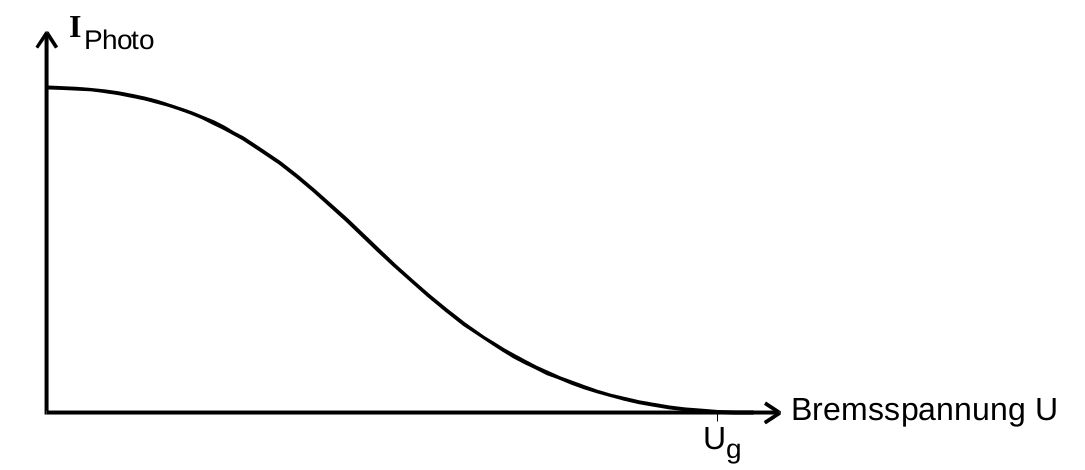
\includegraphics[width=0.90\textwidth]{Bilder/verlauf_photostrom.png}
  \caption{Photostrom in Abhängigkeit zur angelegten Bremsspannung für eine mit monochromatischem Licht bestrahlte Photozelle \cite{Anleitung}.}
  \label{fig:fermidirac}
\end{figure}

In der Realität ist allerdings kein instantaner Abfall bei einer Grenzfrequenz $U_{\mathrm{g}}$
gegeben, sondern ein parabolischer Zusammenhang zwischen dem Strom der ausgelösten Elektronen
und der variablen Spannung $U$ (vergleiche Abbildung \ref{fig:fermidirac}), also
\begin{equation*}
	I_{\mathrm{Ph}} \propto U^2 \mathrm{.}
\end{equation*}
Dies hat den Grund, dass die Elektronen eine Energieverteilung im Metall besitzen. Diese
Energieverteilung wird durch die Fermi-Dirac-Statistik beschrieben, die besagt, dass die
Energie der Valenzelektronen von Null bis zur Fermi-Energie (materialabhängig) verteilt ist.

Ist die benötigte Austrittsarbeit $A_{\mathrm{k}}$ zu groß gegen die Wellenlänge des Lichtes,
muss ein beschleunigendes Potential angelegt werden, damit die Elektronen das Gegenfeld der
Anode überqueren können (vgl. Abbildung \ref{fig:potentialverteilung}).
\begin{figure}
  \centering
  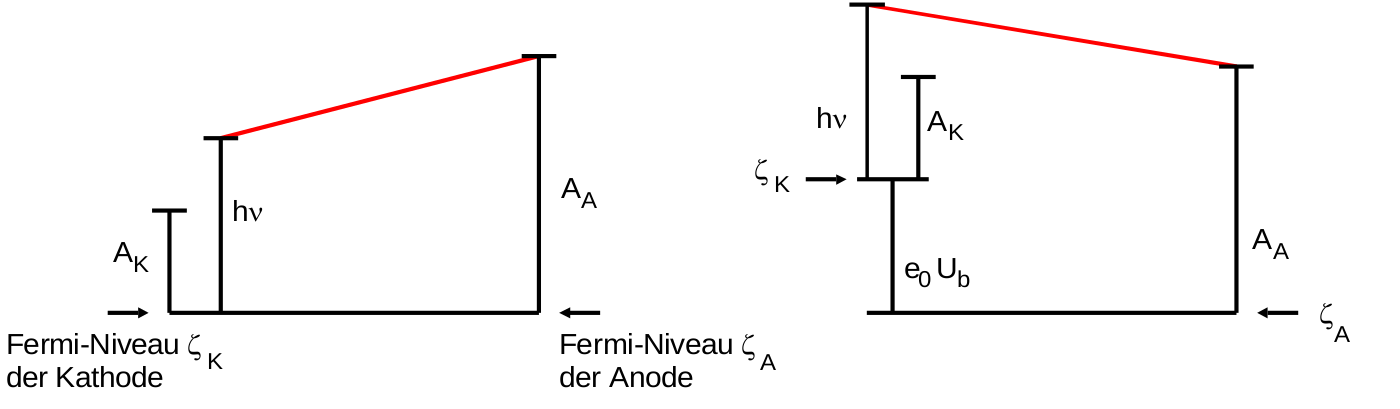
\includegraphics[width=0.90\textwidth]{Bilder/fermi.png}
  \caption{Potentialverhältnisse zwischen Kathode und Anode \cite{Anleitung}.}
  \label{fig:potentialverteilung}
\end{figure}
